\begin{figure}




\end{figure}





% old stuff:
%--------------------------------------
%\begin{figure}
%		\begin{subfigure}{.5\textwidth}
%		  \centering
%	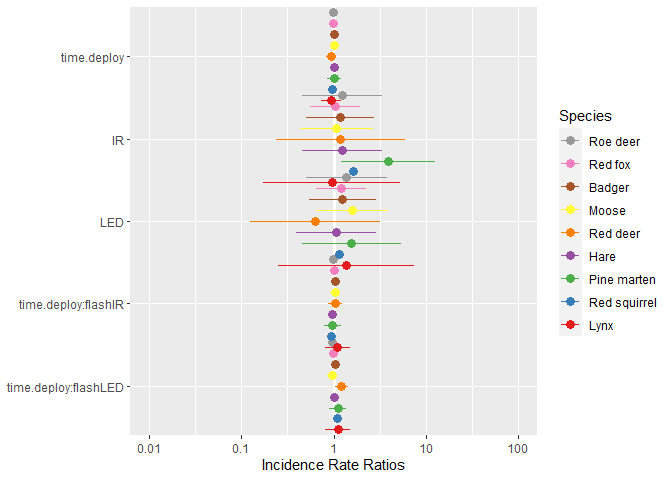
\includegraphics[scale=.7]{../R/glmm_sp_files/figure-html/mod-plot-1.png}
%\caption{Intercept included}
%		\label{fig:para_1}
%	\end{subfigure}
%		\begin{subfigure}{.5\textwidth}
%		  \centering
%	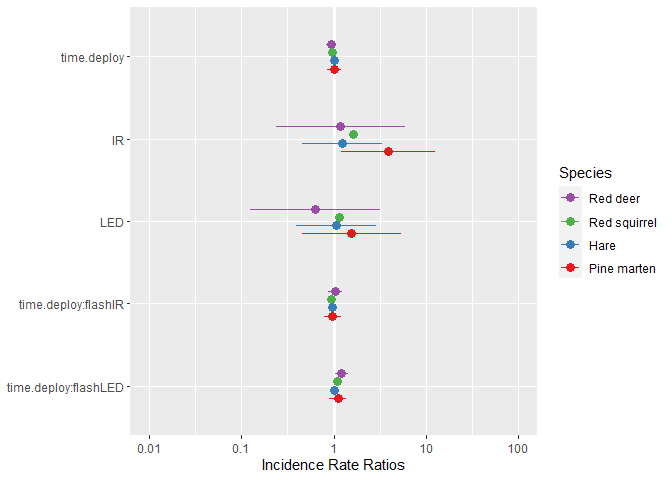
\includegraphics[scale=.7]{../R/glmm_sp_files/figure-html/mod-plot-2.png}
%\caption{with values printed}
%		\label{fig:para_2}
%	\end{subfigure}
%		\caption[Model parameters]%
%    	{Model parameters \par \small Model parameters for all species visualized in joint plots. X axis represents Incidence Rate Ratios (IRR) where 1 signifies a 1:1 ratio with the intercept (flashControl)}
%	\label{fig:para_sp}
%\end{figure}

%___________________________________
%\caption[Marginal effects of GLMMs]
%{Marginal effects of GLMMs \par \small Predicted detection rates of each modelled species. Notice the differing scales of the y axis. Overall, the control-group had no trend over time, and for most species, LED and IR periods weren't significantly different from the control, as their confidence intervals mostly overlap.}

